\begin{figure}[!htb]
\begin{center}
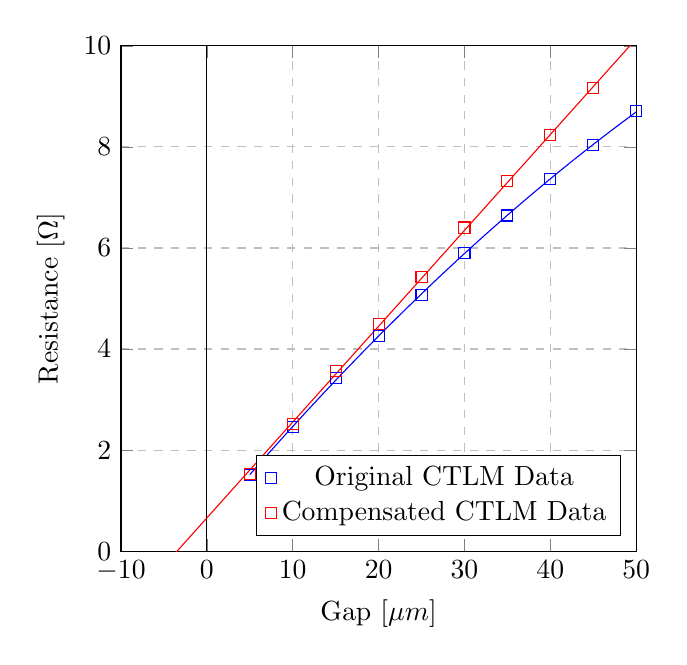
\begin{tikzpicture}

\begin{axis}[
    %title={Temperature dependence of CuSO$_4\cdot$5H$_2$O solubility},
    xlabel={Gap [$\mu m$]},
    ylabel={Resistance [$\Omega$]},
    height=8cm,
    width=0.67\textwidth,
    xmin=-10, xmax=50,
    ymin=0, ymax=10,
    xtick={-10, 0, 10, 20, 30, 40, 50},
    ytick={0, 2, 4, 6, 8, 10},
    % extra y ticks       = 0,
    % extra y tick labels = ,
    % extra y tick style  = { grid = major },
    legend pos=south east,
    ymajorgrids=true,
    xmajorgrids=true,
    grid style=dashed,
]

\addplot[color=blue, mark=square, only marks]
  coordinates {
  (5,1.505363832096823)
  (10,2.449740000726955)
  (15,3.421831099752043)
  (20,4.26394152103118)
  (25,5.070137988413258)
  (30,5.897088680026425)
  (35,6.64208850217324)
  (40,7.356653937259235)
  (45,8.039941315513527)
  (50,8.704528583743103)
};
  \addlegendentry{Original CTLM Data}

\addplot[color=red, mark=square, only marks]
    coordinates {
      (5,1.5245819322833463)
      (10,2.5136557475645573)
      (15,3.5587516564503536)
      (20,4.4966681982956205)
      (25,5.424233303346553)
      (30,6.403332285388977)
      (35,7.323979842935674)
      (40,8.242064238392762)
      (45,9.157502883492521)
      (50,10.085819749510799)
  };
    \addlegendentry{Compensated CTLM Data}

\addplot[color=black]
  coordinates{
    (0,0)
    (0,10)};


\addplot[color=blue,samples=100][domain=5:50]{-0.00077678*x^2 + 0.20218898*x + 0.5225879};

\addplot[color=red,samples=100][domain=-10:50]{0.18961899*x + 0.65853675};

\addplot[color=black] coordinates{(0,0) (10,0)};


\end{axis}
\end{tikzpicture}

\caption{Plot of resistance against CTLM gap size with the as measured data in blue and the data with the correction factor shown in equation \ref{eq:correction} applied shown in red. From the graph $2L_T = 3.473\mu m$ and $2R_c = 0.659\Omega$}
\label{fig:ctlm_res}
\end{center}
\end{figure}
